\chapter{Keretrendszer}

\section{Rendszerarchitektúra áttekintése}

Az áramérzékelők (áramváltó bilincsek) mérik az elektromos áramot és az 
adatokat egy ESP8266 gyűjti, ezek pedig a központi vezérlőhöz táplálják, 
amely vezérlőparancsokat küld visszafelé az elektromos járművek töltőinek 
a megengedett áram beállításához.

Az ESP8266-alapú érzékelőcsomópontok mindegyik elektromos töltőnél el vannak helyezve, 
hogy valós időben mérjék a töltőáramot.
Ezek pedig Wi-Fi-n keresztül küldik el az adatokat egy Python Flask alkalmazást futtató 
vezérlőhöz, amely összesíti a méréseket és kiadja a vezérlőparancsokat.

Maguk az töltők Modbus kommunikációval rendelkeznek, ezért a Modbus protokollon keresztül fogadják a 
távolról érkező utasításokat (esetünkben a megengedett áram beállítását).
Mindegyik töltő saját címmel rendelkezik a soros hálózaton.

Az ESP8266 csomópontok csak az adatok két oldalú továbbadásáért felelősek, aktuális adatokat küldenek a 
szervernek, míg a Flask szerver döntéshozatalt hajt végre és parancsokat ad ki a töltőknek.
Az érzékelés és a vezérlés szétválasztása leegyszerűsíti a végpont tervezését 
és a feldolgozást a szerver oldalon központosítja, ami növeli a robosztusságot.

A Flask szerver egy Prometheus idősoros adatbázissal dolgozik 
(ami külön konténer alapú szolgáltatásként fut), ez naplózza az összes mérést 
a megfigyeléshez és elemzéshez. Az összes kiszolgálóoldali összetevő (a Flask alkalmazás, a Modbus 
interfész és a Prometheus) a Docker használatával van konténerben tárolva a 
felhőalapú környezetben történő egyszerű telepítés érdekében. Az architektúra a 
következőket tartalmazza:

\begin{itemize}
    \item ESP8266 érzékelő csomópontok: 
    Wi-Fi csatlakozású mikrokontrollerek minden végponton (legyen az töltő, megszakító, stb\dots), 
    amelyek a csatlakoztatott érzékelőkön keresztül mérik a váltakozó áramot.
    \item Wi-Fi hálózat: Ami biztosítja, 
    hogy a végpontok tudjanak kommunikálni a központi szerverrel. 
    Mindegyik csomópont csatlakozik a helyi Wi-Fi-hez 
    és HTTPS-kéréseken keresztül adatokat küld a szerver REST API-jának.
    \item Flask alapú központi szerver: 
    Helyi szerveren vagy cloud környezetben is futhat. 
    Mérési adatokat fogad az ESP8266 csomópontoktól, feldolgozza és tárolja azokat 
    és ahogy már említettem Modbus segítségével vezérlőjeleket küld az EV-töltőknek.
    \item Modbus kommunikációs kapcsolat: 
    Összekapcsolja a végpontokat a töltőkkel. Ez esetünkben Modbus/TCP over Ethernet. 
    A végpontok Modbus masterként működnek, és minden elektromos töltő egy Modbus slave eszköz.
    \item Prometheus adatbázis: 
    Idősoros adatbázis, amely összegyűjti és tárolja a mért értékeket 
    (pl. áramok, töltőállapotok, megszakító állapotok) a Flask szerverről valós idejű megfigyeléshez 
    és későbbi elemzéshez.
    \item Docker containerek: 
    A Flask szerver és a Prometheus  Docker-tárolókban fut, 
    így megvalósul a mikroszolgáltatás alapú összeállítás, ami akár helyi szerveren,
    akár modern felhő natív rendszeren jól fut. A Docker biztosítja, hogy az összes szükséges függőséget 
    (Python-könyvtárak stb.) így megkönnyítve az üzemeltetés dolgát, 
    és lehetővé teszi a rendszer megbízható méretezését vagy replikálását.
\end{itemize}

\begin{figure}[ht]
    \centering
    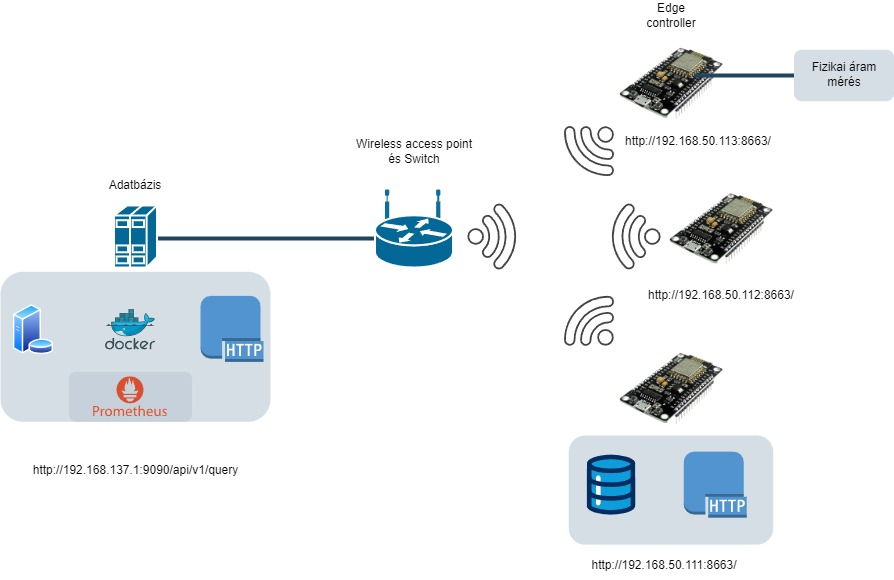
\includegraphics[width=1\textwidth]{figures/szakdoga.jpg}
    \caption{Rendszerarchitektúra}
    \label{fig:Rendszerarchitektúra}
\end{figure}

\section{Eszközök}

\subsection{Végpontok}

\subsubsection{ESP8266 és AC árammérő szenzorok}

A pontos árammérés minden elektromos töltőnél kritikus a rendszer számára. 
Az ESP8266-ot (NodeMCU) nem invazív váltakozóáram-érzékelőkkel 
párosítva használjuk a megfelelő áramkörök által felvett áramerősség mérésére. Egy megfelelő
érzékelő az YHDC SCT-013 sorozatú bilincses áramtranszformátor, például az SCT-013-030 modell, 
ami 30 A AC  feszültségre van méretezve. Az SCT-013 egy osztott magú áramváltó így könnyű a 
csatlakozása, ez a tápkábelnek feszültség alatt 
álló vezetéke köré kerül, és nincs szükség közvetlen elektromos érintkezésre a vezetővel. 
Ez az érzékelő a kábelen átfolyó árammal arányos kis váltakozó feszültséget 
ad ki. Különösen az SCT-013-030 körülbelül 0-1 V AC (effektív) kimenetet produkál 0-30 A mérésekor.
\cite{simplyexplained:emonlib}

\begin{figure}[!ht]
    \centering
    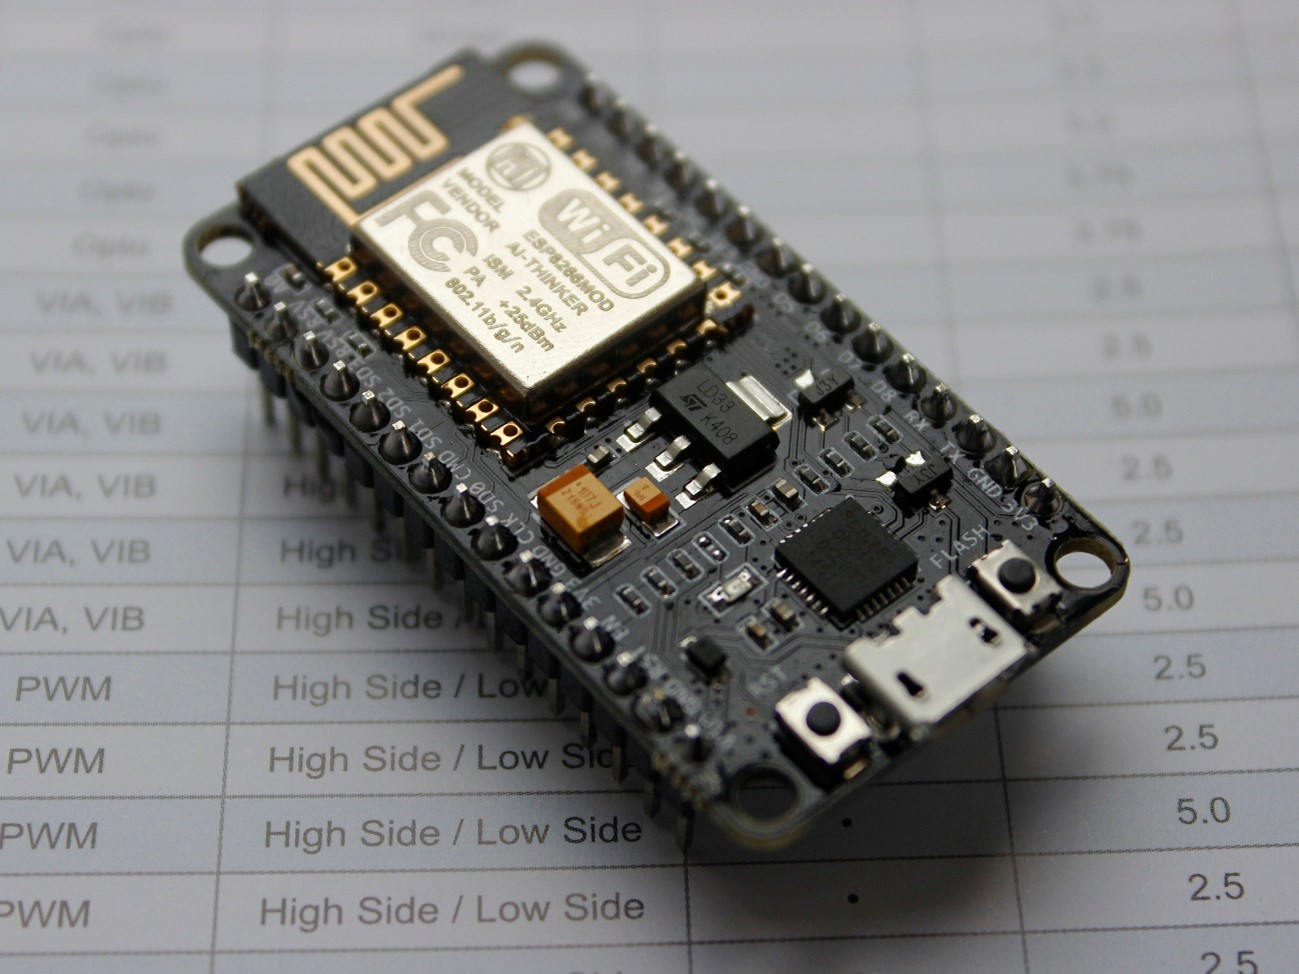
\includegraphics[width=0.8\textwidth, keepaspectratio]{figures/NodeMCU.jpg}
    \caption{NodeMCU (ESP8266) \cite{patel_nodemcu}} 
\end{figure}

Ez a feszültségtartomány kompatibilis az ESP8266 analóg-digitális átalakítójával az analóg bemenetén, 
amely a legtöbb ESP8266 kártyán 0-1 V-ot tud olvasni (a NodeMCU kártyák tartalmaznak beépített 
feszültségosztót, amely lehetővé teszi a 3,3 V-os bemenetet). Így az SCT-013-030 0-1 V-os kimenete 
közvetlenül az analóg bemenetre rakható.
Az SCT-013 érzékelők, amelyek feszültségkimenettel rendelkeznek, 
már rendelkeznek belső ellenállással, így nincs szükség további terhelésre.
\cite{openenergymonitor}

\begin{figure}[!ht]
    \centering
    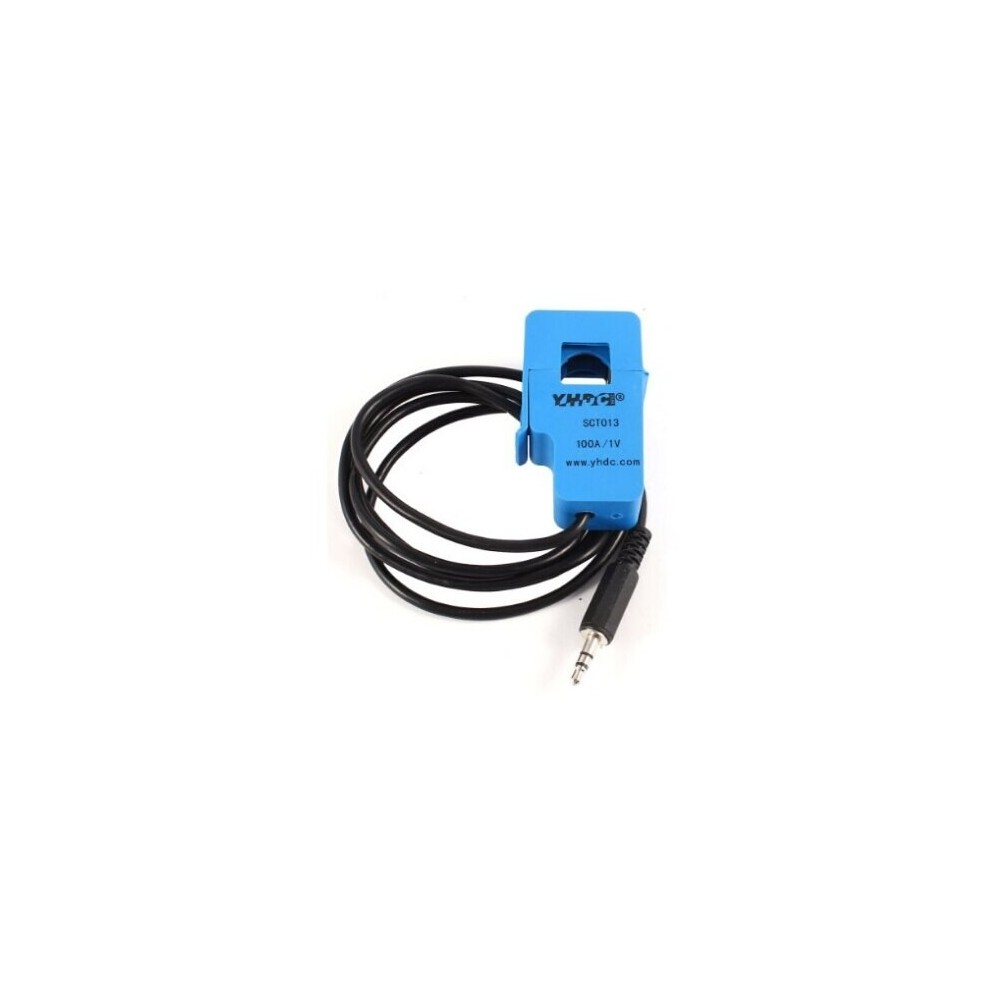
\includegraphics[width=0.8\textwidth, keepaspectratio]{figures/CT.jpg}
    \caption{SCT-013 áramváltó \cite{mikroelektronik:sct013}} 
\end{figure}

Mindkét esetben szükséges egy csatoló áramkör az érzékelőhöz: 
A CT AC kimenete 0 V ha nincsen semmi behatás, de az ESP8266 ADC nem tudja leolvasni a negatív feszültséget. 
Ezért elkell tolnunk az értékeket ehhez kell két ellenállás, amelyek feszültségosztót alkotnak 
a 3,3 V-os tápegységgel, hogy az érzékelő kimenetét a skála közepére rakjuk. 
Lényegében az érzékelő két vezetéke csatlakozik: az egyik az ADC bemenethez, 
a másik pedig a középponthoz körülbelül 1,65 V a 3,3 V-os táp miatt.
\cite{openenergymonitor}

Mindegyik ESP8266 tápellátást kap lehetőleg 5 V-os USB-adapterrel az EV-töltő kiegészítő tápellátásával 
és az analóg bemeneten keresztül olvassa le a CT-érzékelőjét.
A mikrokontroller a megírt kódot futtatja, csatlakozik a Wi-Fi-hez, és folyamatosan méri az áramerősséget. 
Ezt úgy küldi a szervernek, hogy már könnyű legyen prometheusnak tovább küldeni.

\subsubsection{Mért eszközök}

\subsection{Adatbázis}

\subsection{Kontroll szerver}

\section{Kommunikáció}

\subsection{ESP8266 és Szerver között (Wi-Fi és REST API)}

Az adatkommunikációhoz az ESP8266 csomópontok szabványos Wi-Fi hálózatot használnak a mérések továbbítására 
a Flask szerverre. Indításkor minden ESP8266 a tárolt SSID és jelszó használatával csatlakozik a konfigurált 
Wi-Fi hozzáférési ponthoz. A firmware az ESP8266 WiFi könyvtárat használja a hálózathoz való csatlakozáshoz 
(pl. WiFi.begin(ssid, jelszó)), és megvárja, amíg létrejön a kapcsolat
\cite{techtutorialsx:esp8266flask}
. A csatlakozást követően a csomópont képes HTTP kéréseket küldeni a szerver IP-címére. Egy egyszerű RESTful API-t implementálunk a Flask szerveren az adatok fogadásához. Például mindegyik ESP8266 végrehajthat egy HTTP POST kérést egy végponthoz, például a http://<szerver_ip>:5000/api/reading JSON-adattartalommal, amely tartalmazza az aktuális mérést és egy azonosítót. A JSON adatstruktúra a következő lehet:

\subsection{Standardizált Kommunikáció}
